\subsection{Triangles In A Cube}

My dad gave me this problem as a simple problem with a fast answer and said it could be solved within 10 seconds, although I found a way of solving this even faster. I would have expected almost anyone to be able to solve this, although I have been surprised that normal people have pretty poor geometric reasoning abilities. I rate this problem a 1/10 in difficulty.

How many equilateral triangles can be formed by connecting three vertices of a cube?

\textbf{Hints:}

\begin{enumerate}
	\item Connecting any three distinct vertices on the same face will form a right-angled triangle.
	\item Equilateral triangles have rotational symmetry of order 3 - where on a cube do you find such a symmetry?
\end{enumerate}

\textbf{Solution:}

Place three points overlapping at a vertex of the cube. There are three edges connected to this vertex, and we move the points along each of the edges. If all points move along their edge at the same speed then they will form an equilateral triangle by symmetry. Eventually they hit the vertex at the end of the edge, and thus we have found three vertices that form an equilateral triangle. This gives one triangle per vertex, therefore the final answer is 8.

This process is demonstrated in figure~\ref{fig:TrianglesInACube_MovingAwayFromVertex}. The red triangle shows the intermediate step where the points are partially along the edges and the blue triangle shows where it stops. We have not shown that these are the only such triangles, although it is not hard to convince yourself by visualising it. We give more details in the extensions and comments. The next method proves that these are all the equilateral triangles however.

There are 24 orientation-preserving symmetries of the vertices of a cube, and these form the $O$ group. The vertices of an equilateral triangle have 3 orientation-preserving symmetries and form the $C_3$ group. The quotient set $O/C_3$ has size $\left| \frac{O}{C_3} \right| = \frac{|O|}{|C_3|} = \frac{24}{3} = 8$, and this is the number of triples of vertices with threefold rotational symmetry, in other words, the equilateral triangles.

\begin{figure}[H]
	\begin{center}
		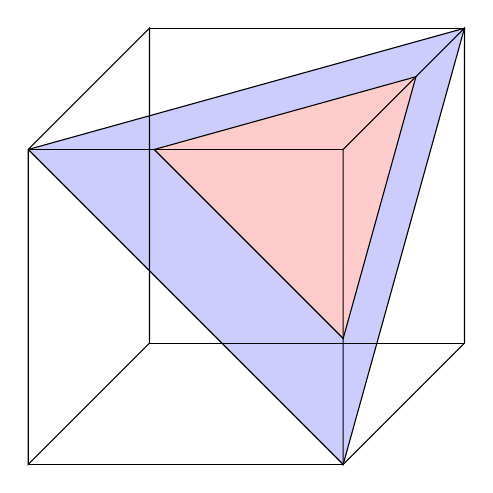
\begin{tikzpicture}[scale=4]
			
			\coordinate (000) at (0, 0, 0);
\coordinate (001) at (0, 0, 1);
\coordinate (010) at (0, 1, 0);
\coordinate (011) at (0, 1, 1);
\coordinate (100) at (1, 0, 0);
\coordinate (101) at (1, 0, 1);
\coordinate (110) at (1, 1, 0);
\coordinate (111) at (1, 1, 1);

			
			\def\d{0.4}
			\coordinate (T1) at (\d, 1, 1);
			\coordinate (T2) at (1, \d, 1);
			\coordinate (T3) at (1, 1, \d);
			
			\filldraw[fill = blue!20] (011) -- (101) -- (110) -- (011);
			\filldraw[fill = red!20] (T1) -- (T2) -- (T3) -- (T1);
			
			\draw (000) -- (001) -- (011) -- (010) -- (000);
\draw (100) -- (101) -- (111) -- (110) -- (100);
\draw (000) -- (100);
\draw (001) -- (101);
\draw (010) -- (110);
\draw (011) -- (111);

			
		\end{tikzpicture}
		\caption{Three points moving away from a vertex at the same speed form an equilateral triangle.}
		\label{fig:TrianglesInACube_MovingAwayFromVertex}
	\end{center}
\end{figure}

\textbf{Extensions and Comments:}

We can confirm that the triangles found that are associated with each vertex are the only such equilateral triangles by considering all possible triangles. Define the distance between two points to be the minimum number of edges of the cube that would need to be traversed to navigate from one to the other. If the three vertices lie within a face of the cube then the triangle must be a right angle and can be eliminated.

Now consider two vertices a distance one apart, that is, on the ends of the same edge. There are three parallel edges. If the remaining vertex is on the two neighbouring edges then the three edges will lie on the same face which has already been covered. If the vertex lies on the diagonally-opposite edge then it will have side lengths of $1$, $\sqrt{2}$, and $\sqrt{3}$, therefore not equilateral.

If the vertices are a distance of three apart then they are on opposite vertices. The third vertex must be within a distance of one of one of the first two vertices and it reduces to a previously given case. All three cases are shown in figure~\ref{fig:TrianglesInACube_Cases}.

\begin{table}[H]
	\centering
	\begin{tabular}{cc}
		\myhline
		Edge lengths & Number of triangles \\
		\myhline
		Live within a face & $4 \cdot 6 = 24$ \\
		Only one edge within a face & $12 \cdot 2 = 24$ \\
		Edges live within three faces & $8$ \\
		Total & ${{8}\choose{3}} = 56$ \\
		\myhline
	\end{tabular}
	\caption{Enumerating all possible triangles formed by connecting vertices of a cube.}
	\label{tab:TrianglesInACube_EnumeratingTriangles}
\end{table}

\begin{figure}[H]
	\begin{subfigure}{0.33\textwidth}
		\centering
		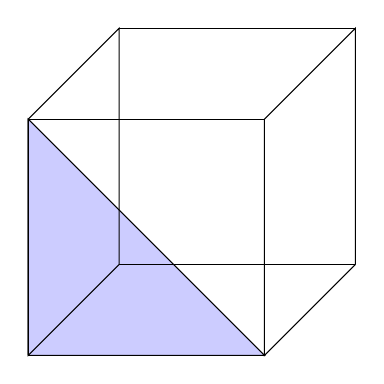
\begin{tikzpicture}[scale=3]
			
			\coordinate (000) at (0, 0, 0);
\coordinate (001) at (0, 0, 1);
\coordinate (010) at (0, 1, 0);
\coordinate (011) at (0, 1, 1);
\coordinate (100) at (1, 0, 0);
\coordinate (101) at (1, 0, 1);
\coordinate (110) at (1, 1, 0);
\coordinate (111) at (1, 1, 1);

			\filldraw[fill = blue!20] (001) -- (101) -- (011) -- (001);
			\draw (000) -- (001) -- (011) -- (010) -- (000);
\draw (100) -- (101) -- (111) -- (110) -- (100);
\draw (000) -- (100);
\draw (001) -- (101);
\draw (010) -- (110);
\draw (011) -- (111);

			
		\end{tikzpicture}
		\caption{Live within a face}
		\label{fig:TrianglesInACube_Case1}
	\end{subfigure}
	\begin{subfigure}{0.33\textwidth}
		\centering
		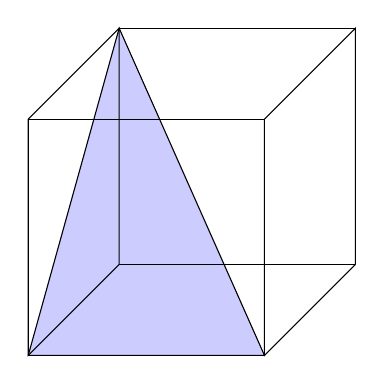
\begin{tikzpicture}[scale=3]
			
			\coordinate (000) at (0, 0, 0);
\coordinate (001) at (0, 0, 1);
\coordinate (010) at (0, 1, 0);
\coordinate (011) at (0, 1, 1);
\coordinate (100) at (1, 0, 0);
\coordinate (101) at (1, 0, 1);
\coordinate (110) at (1, 1, 0);
\coordinate (111) at (1, 1, 1);

			\filldraw[fill = blue!20] (001) -- (101) -- (010) -- (001);
			\draw (000) -- (001) -- (011) -- (010) -- (000);
\draw (100) -- (101) -- (111) -- (110) -- (100);
\draw (000) -- (100);
\draw (001) -- (101);
\draw (010) -- (110);
\draw (011) -- (111);

			
		\end{tikzpicture}
		\caption{Only one edge within a face}
		\label{fig:TrianglesInACube_Case2}
	\end{subfigure}
	\begin{subfigure}{0.33\textwidth}
		\centering
		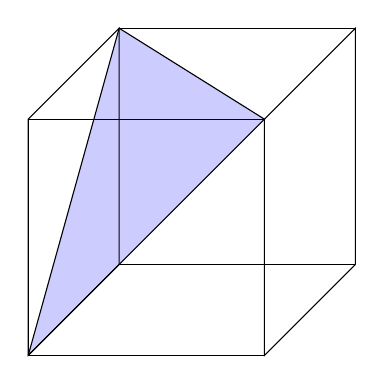
\begin{tikzpicture}[scale=3]
			
			\coordinate (000) at (0, 0, 0);
\coordinate (001) at (0, 0, 1);
\coordinate (010) at (0, 1, 0);
\coordinate (011) at (0, 1, 1);
\coordinate (100) at (1, 0, 0);
\coordinate (101) at (1, 0, 1);
\coordinate (110) at (1, 1, 0);
\coordinate (111) at (1, 1, 1);

			\filldraw[fill = blue!20] (001) -- (111) -- (010) -- (001);
			\draw (000) -- (001) -- (011) -- (010) -- (000);
\draw (100) -- (101) -- (111) -- (110) -- (100);
\draw (000) -- (100);
\draw (001) -- (101);
\draw (010) -- (110);
\draw (011) -- (111);


		\end{tikzpicture}
		\caption{Edges live within three faces}
		\label{fig:TrianglesInACube_Case3}
	\end{subfigure}
	\caption{Examples showing the three ways a triangle can be inscribed within a cube.}
	\label{fig:TrianglesInACube_Cases}
\end{figure}